%%%%%%%%%%%%%%%%%%%%%%% file typeinst.tex %%%%%%%%%%%%%%%%%%%%%%%%%
%
% This is the LaTeX source for the instructions to authors using
% the LaTeX document class 'llncs.cls' for contributions to
% the Lecture Notes in Computer Sciences series.
% http://www.springer.com/lncs       Springer Heidelberg 2006/05/04
%
% It may be used as a template for your own input - copy it
% to a new file with a new name and use it as the basis
% for your article.
%
% NB: the document class 'llncs' has its own and detailed documentation, see
% ftp://ftp.springer.de/data/pubftp/pub/tex/latex/llncs/latex2e/llncsdoc.pdf
%
%%%%%%%%%%%%%%%%%%%%%%%%%%%%%%%%%%%%%%%%%%%%%%%%%%%%%%%%%%%%%%%%%%%
\documentclass[runningheads]{llncs}
%\usepackage[dvips]{color}
%\usepackage{multicol}
%\usepackage{tabls}
%\usepackage{ttbox}
\usepackage{allmtt}
%\usepackage{pstricks,pst-node,pst-tree} % PS Tricks for diagrams
%\usepackage{proof2}
\setcounter{tocdepth}{3}
\usepackage{graphicx}
\usepackage{amsmath}
\usepackage{amssymb}
\usepackage{latexsym}
\usepackage{stmaryrd}
%\usepackage{mbboard}
\usepackage{xspace}
%\usepackage{diagrams}

\usepackage{url}
\urldef{\mailsa}\path|l.dixon@ed.ac.uk|
\urldef{\mailsb}\path|ross.duncan@comlab.ox.ac.uk|
\newcommand{\keywords}[1]{\par\addvspace\baselineskip
\noindent\keywordname\enspace\ignorespaces#1}

% -=-=-=-=-=-=-=-=-=-=-=-=-=-=-=-=-=-=-=-=-=-=-=-=-=-=-=-=-=-=-=-=-=-=-=-=-
%   Random maybe useful things...
% -=-=-=-=-=-=-=-=-=-=-=-=-=-=-=-=-=-=-=-=-=-=-=-=-=-=-=-=-=-=-=-=-=-=-=-=-
\newcommand{\cmnt}[1]{\textcolor[rgb]{ 0.8,      0,    0  }{#1}}
%\newcommand{\intabp}[2]{\parbox[t]{#1}{\raggedright{#2}\vspace{0.2cm}}}
%\newcommand{\vsmall}[1]{\footnotesize{#1}}
\newcommand{\ors}{\oplus}
\newcommand{\tensor}{\otimes}

%%-----------------------------------------------------------------
%%%% Ross's handy macros %%%%%%%%%%%%%%%%%%%%%%%%%%%%%%%%%%%%%%%%%%
%%-----------------------------------------------------------------

\newcommand{\figureline}{\rule{\textwidth}{0.5pt}}
\newcommand{\figureend}{\rule{\textwidth}{0.5pt}}

\newcommand{\dimm}{\mathrm{dim}}

% aliases
\newcommand{\infinity}{\infty}
\newcommand{\iso}{\cong}
\newcommand{\isomorphism}{\cong}

% ``semantic'' brakets
\newcommand{\denote}[1]{% ---------
\llbracket #1 \rrbracket} 
% name / coname 
\newcommand{\name}[1]{%--------
\ulcorner #1 \urcorner}
\newcommand{\coname}[1]{%
\llcorner #1 \lrcorner}

\newcommand{\sizeof}[1]{% \sizeof{x} == |x|
  \left|#1\right|}


%-------------------------------------------------------
%  Useful macros for all things categorical
%-------------------------------------------------------

\newcommand{\dom}{\operatorname{dom}}
\newcommand{\cod}{\operatorname{cod}}
\newcommand{\Tr}{\operatorname{Tr}}

% Objects of ???
\newcommand{\OBJ}[1]{\ensuremath{\mathrm{Obj}_{#1}}}
%
% Objects of {\cal ??}
\newcommand{\OBJC}[1]{\ensuremath{\mathrm{Obj}_{{\cal #1}}}}

%
% Arrows of ???
\newcommand{\ARR}[1]{\ensuremath{\mathrm{Arr}_{#1}}}
%
% Arrows of {\cal ??}
\newcommand{\ARRC}[1]{\ensuremath{\mathrm{Arr}_{{\cal #1}}}}


% Caligraphic category names
\newcommand{\catA}{\ensuremath{{\cal A}}\xspace}
\newcommand{\catB}{\ensuremath{{\cal B}}\xspace}
\newcommand{\catC}{\ensuremath{{\cal C}}\xspace}
\newcommand{\catD}{\ensuremath{{\cal D}}\xspace}
\newcommand{\catE}{\ensuremath{{\cal E}}\xspace}
\newcommand{\catF}{\ensuremath{{\cal F}}\xspace}
\newcommand{\catG}{\ensuremath{{\cal G}}\xspace}
\newcommand{\catH}{\ensuremath{{\cal H}}\xspace}
\newcommand{\catP}{\ensuremath{{\cal P}}\xspace}
\newcommand{\catQ}{\ensuremath{{\cal Q}}\xspace}

%sub scripted identity morphisms
\newcommand{\id}[1]{\ensuremath{\mathrm{id}_{#1}}}

% Boldified names of useful categories
%
\newcommand{\vectfd}[1]{% category of finite dimensional vector spaces over some field
\ensuremath{\textbf{Vect}^{\mathrm{fd}}_{#1}}\xspace}
\newcommand{\vectfdc}{% category of finite dimensional vector spaces over complexes
\vectfd{\mathbb{C}}}
\newcommand{\catRel}{% the category of sets and relations
\ensuremath{\textbf{Rel}}\xspace}
\newcommand{\catSet}{% the category of sets and functions
\ensuremath{\textbf{Set}}\xspace}
\newcommand{\catCat}{% the category of (small) categories
\ensuremath{\textbf{Cat}}\xspace}
\newcommand{\catInvCat}{% the category of involutive categories
\ensuremath{\textbf{InvCat}}\xspace}
\newcommand{\catComCl}{% the category of compact closed  categories
\ensuremath{\textbf{ComCl}}\xspace}
\newcommand{\catSComCl}{% the category of strongly compact closed  categories
\ensuremath{\textbf{SComCl}}\xspace}
\newcommand{\catGrph}{% the category of graphs
\ensuremath{\textbf{Grph}}\xspace}
\newcommand{\qubit}{% the category of qubits
\ensuremath{\textbf{Qubit}}\xspace}
\newcommand{\fdhilb}{% the category of finite dimensional hilbert space
\ensuremath{\textbf{FDHilb}}\xspace}
\newcommand{\catInvCom}{% the category of involutive categories
\ensuremath{\textbf{InvCom}}\xspace}
\newcommand{\catCom}{% the category of compact closed  categories
\ensuremath{\textbf{Com}}\xspace}
%%%% End of Ross's lovely categorcal macros--------

%%%%  use this to include graphics in the right place.
\newcommand{\inlinegraphic}[2]{
  %% todo -- make this thing calculate the height 
  %% itself based on a global scaling factor
  \dimendef\grafheight=255\dimendef\grafvshift=254
  \grafheight=#1
  \grafvshift=-0.5\grafheight
  \advance\grafvshift by 0.5ex
  \raisebox{\grafvshift}{\includegraphics[height=\grafheight]{images/#2}\xspace}
}



%%--------------------------------------------

\begin{document}

\mainmatter  % start of an individual contribution

% first the title is needed
\title{Reasoning Graphically about Quantum Computation}

% a short form should be given in case it is too long for the running head
%\titlerunning{Reasoning Graphically about Quantum Computation}

% the name(s) of the author(s) follow(s) next
%
% NB: Chinese authors should write their first names(s) in front of
% their surnames. This ensures that the names appear correctly in
% the running heads and the author index.
%
\author{Lucas Dixon\inst{1} \and Ross Duncan\inst{2}~\thanks{EPSRC Grants...}%
}
%
%\authorrunning{Lecture Notes in Computer Science: Authors' Instructions}
% (feature abused for this document to repeat the title also on left hand pages)

% the affiliations are given next; don't give your e-mail address
% unless you accept that it will be published
\institute{\mailsa, University of Edinburgh
\and \mailsb, University of Oxford
%\mailsa\\
%\mailsb\\
%\mailsc
}

%
% NB: a more complex sample for affiliations and the mapping to the
% corresponding authors can be found in the file "llncs.dem"
% (search for the string "\mainmatter" where a contribution starts).
% "llncs.dem" accompanies the document class "llncs.cls".
%
%\toctitle{Lecture Notes in Computer Science}
%\tocauthor{Authors' Instructions}
\maketitle


\begin{abstract}
  Systems of quantum computation are typically represented by large
  matrix compositions. However, recent graph-based formalisms offer an
  approach which exposes the structure of these systems in a clearer
  and more accessible way. Although these provide a significantly
  simpler way of reading and presenting quantum computations, manual
  manipulation of such graphs is slow and error prone. We
  present a formalism that supports a mechanised reasoning about such
  graphs. This involves a compositional account of graph rewriting
  that preserves the underlying categorical semantics. We present a
  system, which has been implemented, with a fixed logical kernel and
  support for derived rules, which allows the model of quantum
  computation  to be specified declarativley.
  Soundness of the 
  system is proved with respect to the underlying model and
  completeness is an open problem.

  \keywords{graph rewriting, quantum computing, categorical
    logic, interactive theorem proving, graphical calculi}
\end{abstract}


\section{Introduction}
\label{sec:introduction}

\section{Compact Closed Categories and Graphs}
\label{sec:mono-categ-graphs}

representation of freely generated compact closed  categories  as
graphs;

theorem: two arrows in a a freely generated compact closed  category
are equal iff and only if their graphs are equal.

Note that the notion of vertex and graph have the same external
structure so it is possible to view a subgraph as a vertex and vice versa.

\section{Quotients and Rewriting}
\label{sec:quotients-rewriting}

Few examples of interesting compact closed categories are freely
generated.  In practice we work with categories presented as
generators and \emph{equations}.  For 
representing quantum computations, Coecke and Duncan
\cite{Coecke:2008jo} propose the following collection of generators:
\begin{description}
\item[Objects] the self dual object $Q$;
\item[Arrows] Two families of arrows:
  \begin{align}
  &\epsilon_Z : Q \to I, &\qquad&  \epsilon_X : Q \to I,\\
  &\delta_Z : Q \to Q \otimes Q, && \delta_X : Q \to Q \otimes Q, \\
  &\alpha_Z : Q \to Q &&  \alpha_X : Q \to Q   
  \end{align}
  where $\alpha \in [0,2\pi)$, and in addition $H:Q\to Q$.
\end{description}
We represent these two families, and their adjoints, by colours in our
graphical notation:
\begin{gather*}
  \epsilon_Z = \inlinegraphic{1.5em}{epsilon} \qquad
  \delta_Z = \inlinegraphic{1.5em}{delta} \qquad
  \epsilon_Z^\dag = \inlinegraphic{1.5em}{epsilondag} \qquad
  \delta_Z^\dag = \inlinegraphic{1.5em}{deltadag} \qquad
  \alpha_Z = \inlinegraphic{1.5em}{greenalpha} \qquad
\\  
  \epsilon_X = \inlinegraphic{1.5em}{redepsilon} \qquad
  \delta_X = \inlinegraphic{1.5em}{reddelta} \qquad
  \epsilon_X^\dag = \inlinegraphic{1.5em}{redepsilondag} \qquad
  \delta_X^\dag = \inlinegraphic{1.5em}{reddeltadag} \qquad
  \alpha_X = \inlinegraphic{1.5em}{redalpha} \qquad
\end{gather*}
The $H$ arrow is denoted by \inlinegraphic{1.5em}{H}.  The free
compact closed category  is then given by all graphs formed by
composing and tensoring these basic graphs.

To model the behaviour of quantum systems certain additional equations
must be satisfied.  Each family $(\delta, \epsilon)$ must form a
\emph{classical structure}
\cite{Coecke2006Quantum-Measure,Coecke2006POVMs-and-Naima}:  the pair
$(\delta, \epsilon)$  should form a cocommuative comonoid, the pair
$(\delta^\dag,\epsilon^\dag)$ must form a commutative monoid, and
together they must satisfy the isometry and frobenius equations. In
addition the family $\alpha$ must form an abelian group with $\alpha^\dag
= -\alpha$.  These equations are presented graphically below for the
green family;  the red vertices obey all the same equations
\begin{description}
\item[Comonoid Laws] 
\[
\begin{array}{ccccccccccccccc}
  \inlinegraphic{3.5em}{comonoid-assoc1}  &=\;&
  \inlinegraphic{3.5em}{comonoid-assoc2}
  &\qquad\qquad&
  \inlinegraphic{3.7em}{comonoid-unit1}  &=\;&
  \inlinegraphic{3.7em}{comonoid-unit2}  &=\;&
  \inlinegraphic{3.7em}{comonoid-unit3} 
  &\qquad\qquad&
  \inlinegraphic{3.5em}{comonoid-comm1}  &=\;&
  \inlinegraphic{3.5em}{comonoid-comm2}
\end{array}
\]
\item[Monoid Laws] 
\[
\begin{array}{ccccccccccccccc}
  \inlinegraphic{3.5em}{monoid-assoc1}  &=\;&
  \inlinegraphic{3.5em}{monoid-assoc2}
  &\qquad\qquad&
  \inlinegraphic{3.7em}{monoid-unit1}  &=\;&
  \inlinegraphic{3.7em}{monoid-unit2}  &=\;&
  \inlinegraphic{3.7em}{monoid-unit3} 
  &\qquad\qquad&
  \inlinegraphic{3.5em}{monoid-comm1}  &=\;&
  \inlinegraphic{3.5em}{monoid-comm2}
\end{array}
\]
\item[Isometry] 
\item[Frobenius]
  \[
  \begin{array}{ccccc}
    \inlinegraphic{3.5em}{frobenius1}  &=\;&
    \inlinegraphic{3.5em}{frobenius2} &=\;&
    \inlinegraphic{3.5em}{frobenius3}
  \end{array}
  \]
  \item[Abelian Unitary Group]
\end{description}

Each family $(\delta, \epsilon, \alpha)$ is governed by a set of
equations defining a forms a \emph{classical structure}
 with a
\emph{phase group}.  The requisite equations state that $(\delta,
\epsilon )$ form a cocommutative comonoid:
\begin{gather}
  (\delta \otimes \id{Q}) \circ \delta 
   =   ( \id{Q} \otimes \delta) \circ \delta  
  \tag{A}\label{comonoid-assoc}
  \\
  (\epsilon \otimes \id{Q}) \circ \delta 
  = (\id{Q} \otimes \epsilon)\circ \delta 
  = \id{Q} \tag{U} \label{comonoid-unit}
  \\
  \delta = \sigma \circ \delta. \tag{C}\label{comonoid-comm}
\end{gather}
Their adjoints $(\delta^\dag,\epsilon^\dag)$ form a commutative
monoid':
\begin{gather}
  \delta^\dag \circ (\delta^\dag \otimes \id{Q})
  =    \delta^\dag   \circ ( \id{Q} \otimes \delta^\dag) 
  \tag{A}\label{monoid-assoc}
  \\
  \delta^\dag  \circ (\epsilon^\dag \otimes \id{Q}) 
  = \delta^\dag \circ (\id{Q} \otimes \epsilon^\dag)
  = \id{Q} \tag{U} \label{monoid-unit}
  \\
  \delta^\dag = \delta^\dag \circ
  \sigma. \tag{C}\label{monoid-comm}.
\end{gather}
Futher, these jointly satisfy the \emph{isometry} and \emph{frobenius} laws:
\begin{gather}
  \delta^\dag \circ \delta = \id{Q} \tag{I}\label{isometry}
  \\
  (\delta^\dag \otimes \id{Q}) \circ (\id{Q}\otimes \delta)
  = \delta \circ \delta^\dag. \tag{F}\label{frobenius}
\end{gather}


The need to formalise these equations leads naturally to a rewriting
theory 

\section{Graph Patterns}
\label{sec:patterns}

The representation of Compact Closed Categories as Graphs, discuseed
in the previous section, is too restrictive for automated reasoning
about quantum computation. In particular, pictures such as the
following are frequently needed:

\begin{center}
  \scalebox{1.0}{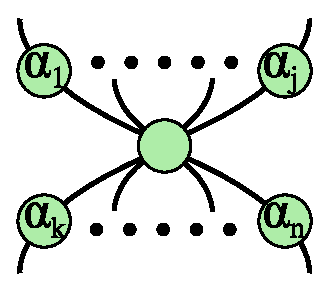
\includegraphics{images/spider_lhs}}
\end{center}

\noindent Such pictures represent an infinite family of concrete
graphs. In this section we describe an extension of the representation
for Compact Closed Categories that allows a graph-based representation
that captures an infinite family of graphs. Notably, this allows us to
represent laws about quantum computation, such as
Spider-Law~\ref{spider-law-fig}. Furthermore, this representation is
still compositional in the sense that we can compose graphs. The
extension, which we call \ref{graph patterns}, adds two extra kinds of
nodes to the graph. Namely, {\em banged boxes} which informally
represent an arbitrary number of copies of a node (where the node is
defined as some graph), and {\em variable nodes} which informally
represent some, as yet unkown, node in a graph.

\subsection{!-Boxes}

!-Boxes 

\subsection{Variable Nodes}

In graph patterns, variable nodes generalise the concept of a
half-edge. Variable nodes, unlike boundary-nodes in the concrete
graph, are not classified into domain and co-domain. The intuition of
a variable node is that it can be replaced by any concrete node. Thus,
unlike nodes in conrete a graph, variable node's do not define an
ordering on the edges that are incident. Instead, the edges that touch
a variable node are simply a set.

The type of a variable nodes is thus defined as a multiset rather than
a tensor. Any tensor type can be lifted into a multiset type in the
obvious manner, which we denote by the operation {\tt
  mset\_of\_tensor}. For example, {\tt mset\_of\_tensor($a \tensor b
  \tensor a$) = $\{(a,2), (b,1)\}$}. We say that a tensor-type, $T$,
is an instance of a multiset type, $M$, when it's lifting into a
multiset is a super-set of $M$: $ M \subseteq
\mathtt{mset\_of\_tensor}(T) \Longrightarrow T \in M$. The intuition
here is that an instance of variable node is allowed to have as many
extra edges as it likes as long as it at least has the ones mentioned
in the original graph. A variable node, $a$ is be said to an instance
of another variable node $b$ when the multiset represnting the type of
$a$ is a superset of the multiset for the type of $b$. Thus, with
regard to the underlying semantics, $a$ being a subtype of $b$ means
that the set of instances of $a$ are a subset of the instances of $b$.

\begin{figure}[t]
%  \scalebox{1.0}{\includegraphics{images/node-var-instance.eps}}
*** Add figure *** 
\label{node-variable-instances-fig}\caption{The concrete graphs $a$,
  $b$, and $c$ are instances of $x$, a graph with variables nodes.}
\end{figure}

A graph with variable nodes is given a formal semantics by being
interpretated as a set of concrete graphs. We refer members of
interpretation set as instances. Formally, an instance of a graph with
variable-nodes is the graph where every variable node has been
replaced by some instance of it. For example, in
Figure~\ref{node-variable-instances-fig}, the graphs $a$, $b$ and $c$
are instances of the graph $x$. Observe that when a variable-node has
degree one, then it can be instantiated as a boundary edge of either
the domain or co-domain. 

\subsection{Compositonality}

In this section, we define a compositonality principle for graphs
patterns, that is graphs with variable-nodes and !-boxes. This is
related to compositionality of the underlying concrete graphs by the
following instantiation homomorphism:



By enriching graphs with to form
graph-patterns, we need to define compositionality principle from the
underlying concrete graphs. In this section, we restore
compositionality and show its correspondence to the underyling
principle in concrete graphs.

Definition: super-type: given a node with type T

Type Expressions: we introduce a new form of type for a pattern
graph. In particular, a variable node with 


\subsection{Instantiation}



\section{Graph Pattern Rewriting}
\label{sec:rewriting}

\subsection{Rules}
\subsection{Unification}
\subsection{Substitution}


\section{Node Expressions}
\label{sec:node-expressions}


\section{Related Work}
\label{sec:relatedwork}

Initially one might be tempted to think that the usual notion of
subgraph might surfice for expressing matching, however it allows
additional edges on nodes where, because of the tensorial semantics of
our graphs, we do not. Our work provides a restriction of the usual
subgraph definition that is sound for Compact Closed Categories.

Link Graphs and their extention to BiGraphs also encapsualte a very
different kind of semantics where they allow edges to go to multiple
nodes. An interesting area of further work would be to consider our
graph patterns for these, and other, graph based formalisms.

Graph Grammars...

Other graph rewriting... 

Matrix Based Graph Tansformation...

Other Graph Transformation...

\section{Conclusions}
\label{sec:conclusions}

Ideas for further work
\begin{itemize}
\item simplification ordering
\item confluence arguments for graphs
\item formalise algorithms in a thm prover
\item richer graph structures - quantification over edges
\item richer expression language in vertices
\item completeness of rewrite rules with respect to wpHilb
\end{itemize}

\bibliographystyle{plain}
\bibliography{all}
\bibliography{bibfile}

\end{document}



